\documentclass[border=10pt]{standalone}
\usepackage{tikz}
\usetikzlibrary{automata, positioning, arrows.meta}

\begin{document}
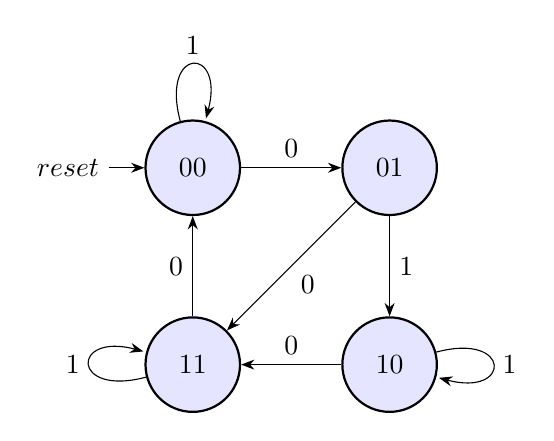
\begin{tikzpicture}[
    ->, >=Stealth, auto, node distance=2.5cm,
    every state/.style={thick, fill=blue!10, minimum size=1.2cm},
    initial text=$reset$
]

    % States
    \node[state, initial] (s00) {00};
    \node[state, right of=s00] (s01) {01};
    \node[state, below of=s01] (s10) {10};
    \node[state, below of=s00] (s11) {11};

    % Transitions
    \path (s00) edge[loop above] node {1} (s00)
                edge node {0} (s01);
                
    \path (s01) edge node {0} (s11)
                edge node {1} (s10);
                
    \path (s10) edge[loop right] node {1} (s10)
                edge node[above] {0} (s11);
                
    \path (s11) edge[loop left] node {1} (s11)
                edge node {0} (s00);

\end{tikzpicture}
\end{document}
